%نام و نام خانوادگی:
%شماره دانشجویی: 
\مسئله{پارسر LALR(1)}

\پاسخ{
\begin{enumerate}
	\item
	
		\begin{figure}[H]
			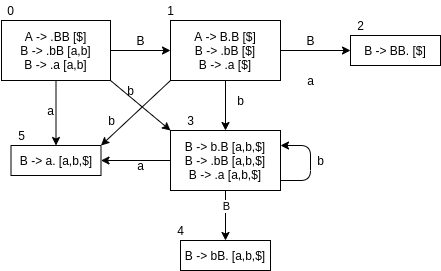
\includegraphics[width=\linewidth]{./commons/Q9.png}
			\label{fig:Q6}
		\end{figure}
		\lr{
		\begin{table}[H]
			\begin{tabular}{c|c|c|c|c}
				 & a   & b   & \$  & B  \\
				 \hline
				 0 & S5 & S3 & & 1\\
				 1 & S5 & S3 & & 2\\
				 2 &  &  & R1 & \\
				 3 & S5 & S3 & & 4\\
				 4 & R2 & R2 & R2 & \\
				 5 & R3 & R3 & R3 & \\
				\hline
			\end{tabular}
		\end{table}
		}
می‌خواهیم رشته ‌babba را پارس کنیم. مشابه سوال قبل عمل می‌کنیم.
\lr{
\\0 -> b > 3 > a -> 5 , look a head = b
\\0 -> b -> 3 -> B -> 4 , look a head = b
\\0 -> B - > 1 -> b -> 3 -> b -> 3 ->  a -> 5 , look a head =\$
\\0 -> B - > 1 -> b -> 3 -> b -> 3 -> B -> 4 , look a head =\$
\\0 -> B - > 1 -> b -> 3 -> B -> 4 , look a head = \$
\\0 -> B - > 1 -> B ->2 , look a head = \$
\\0 -> A -> \$ -> acc
}
\end{enumerate}
}